% ─────────────────────────────────────────────────────────────────────────────
% AdmitGPT — Research Paper (IEEE Conference format)
% Author: Ziad Salah — Independent Researcher
% Language: English. Content grounded in the implemented engine; proposed
% mechanisms are explicitly flagged as Future Work (see Sec. V).
% Compile with: pdflatex + bibtex + pdflatex + pdflatex  (uses local ./ieee/IEEEtran)
% ─────────────────────────────────────────────────────────────────────────────
\documentclass[conference]{IEEEtran}

\usepackage[utf8]{inputenc}
\usepackage{amsmath,amssymb,amsfonts}
\usepackage{graphicx}
\usepackage{textcomp}
\usepackage{xcolor}
\usepackage{url}
\usepackage{cite}
\usepackage{tikz}
\usetikzlibrary{shapes.geometric, arrows.meta, positioning, fit, calc}

\hyphenation{ad-mis-sions asym-me-try de-ter-min-is-tic client-side ana-lyt-ics}

\begin{document}

\title{An Open-Source Deterministic Framework for Mitigating Information Asymmetry in University Admissions Analytics}

\author{
\IEEEauthorblockN{Ziad Salah}
\IEEEauthorblockA{Independent Researcher\\
Email: zs.01117875692@gmail.com}
}

\maketitle

\begin{abstract}
Getting into college has turned into a game where the people with the data---schools and the consultants who advise applicants---know far more about what actually works than the applicants themselves. This paper describes AdmitGPT, an open-source engine that runs entirely in the browser and computes admission odds deterministically instead of hiding the math behind a black box. It loads a 5.2\,MB dataset of 1,122 historical profiles and runs an open additive-logistic engine with no server-side data collection. We spell out the parts that matter: a single logistic model in which academic strength, a six-factor Spike model for extracurriculars and awards, a Renaissance bonus for students who work across unrelated fields, and major-fit and international modifiers each contribute additively to the admission log-odds, with a hard cap on the spike term, a verification-aware discount that dampens unverified over-claiming, and native-scale GPA reconciliation for international applicants. We report an exploratory calibration study on 11,658 academic-only student-school pairs and a full-engine evaluation on 11,685 pairs in which the missing spike fields are derived heuristically from the free-text extracurricular descriptions. The academic-only path discriminates observed outcomes with AUC 0.7383 (Brier 0.2848); the full engine reaches AUC 0.7398 (Brier 0.2762), so the heuristically derived spike leaves discrimination essentially unchanged over academics while improving absolute calibration on this corpus. Both are moderate discriminative signals with imperfect absolute calibration, and they are single-corpus exploratory checks rather than held-out validations; the engine's predictive value under genuine structured spike inputs remains untested. The engine is released on GitHub with its calibration scripts and is fully reproducible~\cite{admitgpt}. The signed deterministic report is deliberately incomplete: it serves as a grounding layer for an external evaluator (an LLM the user trusts, a human specialist, or both) that reads the full application narrative---essay, context, personal story---alongside the auditable math. The mathematical anchor constrains hallucination in LLM-based evaluation and provides a verifiable baseline for human judgment, while the narrative layer captures what numbers cannot. We close with a plan for improving the data without giving up privacy: spike-annotated held-out evaluation, anonymized verification surveys, and federated university alliances.
\end{abstract}

\begin{IEEEkeywords}
information asymmetry, admissions analytics, deterministic models, client-side computing, privacy-by-design, transparency, black-box mitigation.
\end{IEEEkeywords}

% ─────────────────────────────────────────────────────────────────────────────
\section{Social Impact and the Philosophical Framing}
\subsection{The Information Asymmetry Problem}
The core problem is an information gap. Schools and the consultants who advise applicants know a lot more about historical outcomes than the applicants do, and that gap is worth real money. Akerlof's work on markets with quality uncertainty makes the point generally~\cite{akerlof}: when one side holds the information, the other side gets exploited. Admissions consulting runs on exactly this---hundreds of dollars an hour for access to acceptance rates, yield patterns, and holistic rubrics that are, in principle, public information. The applicant pays because the actual math is never shown.

\subsection{The Transparency Manifesto}
AdmitGPT takes the opposite stance: show everything. Every formula, weight, and known limitation is in the source, and the app has a page that walks through the math for each result. The point is simple---give the same inputs and you get the same outputs, and anyone who can read code can check the numbers themselves.

\subsection{Core Contributions}
What this paper actually contributes:
\begin{enumerate}
    \item An additive-logistic scoring architecture in which academics, the Spike model, and modifiers contribute to a single admission logit, with a cap that lets genuine outliers stand out without letting one achievement overpower weak grades.
    \item A privacy-first design where all computation happens in the browser, so no minor's data has to be collected or stored.
    \item A report-signing scheme (AES-256) that ties each output to its inputs, so a result can be checked without exposing who the applicant is.
    \item An exploratory calibration study on 11,658 academic-only and 11,685 full-engine student-school pairs. The academic-only path reaches AUC 0.7383 (Brier 0.2848); the full engine with heuristically derived spike reaches AUC 0.7398 (Brier 0.2762). The spike contributes no measurable discrimination lift over academics on this corpus, but improves absolute calibration, and the engine's predictive claims remain exploratory, single-corpus, and unvalidated.
\end{enumerate}

% ─────────────────────────────────────────────────────────────────────────────
\section{Engine Architecture and Mathematical Formulation}
\subsection{System Pipeline Overview}
Fig.~\ref{fig:pipeline} summarizes the data flow. The historical dataset (student profiles, college metadata, computed statistics) is fetched once and held in browser memory. The user's profile is combined with the dataset to (i) compute academic Z-scores, (ii) run a k-NN cluster to locate the nearest accepted and rejected peers, (iii) compute the Spike score, and (iv) evaluate the additive-logistic probability. No field of the user's profile is transmitted to any external server; the only network egress is the optional, user-initiated dispatch of an outlier invitation message to a private datastore.

\begin{figure}[!t]
\centering
\resizebox{\columnwidth}{!}{%
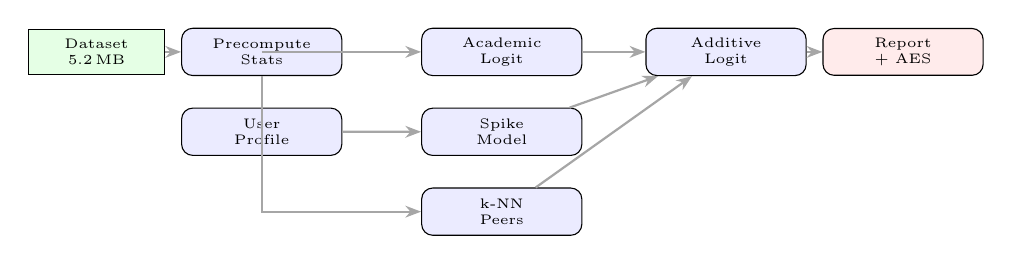
\begin{tikzpicture}[
    node distance=0.4cm and 0.2cm,
    block/.style={rectangle, draw, fill=blue!8, text width=1.8cm, text centered, rounded corners, minimum height=0.6cm, font=\tiny},
    data/.style={rectangle, draw, fill=green!10, text width=1.5cm, text centered, minimum height=0.5cm, font=\tiny},
    output/.style={rectangle, draw, fill=red!8, text width=1.8cm, text centered, rounded corners, minimum height=0.5cm, font=\tiny},
    arrow/.style={-{Stealth[length=2mm]}, thick, color=gray!70},
]
\node[data] (dataset) {Dataset\\5.2\,MB};
\node[block, right=of dataset] (stats) {Precompute\\Stats};
\node[block, below=of stats] (profile) {User\\Profile};
\node[block, right=of stats, xshift=0.8cm] (gate) {Academic\\Logit};
\node[block, below=of gate] (spike) {Spike\\Model};
\node[block, below=of spike] (knn) {k-NN\\Peers};
\node[block, right=of gate, xshift=0.6cm] (combine) {Additive\\Logit};
\node[output, right=of combine] (report) {Report\\+ AES};
\draw[arrow] (dataset) -- (stats);
\draw[arrow] (stats) |- (gate);
\draw[arrow] (profile) -- (spike);
\draw[arrow] (stats) |- (knn);
\draw[arrow] (gate) -- (combine);
\draw[arrow] (spike) -- (combine);
\draw[arrow] (knn) -- (combine);
\draw[arrow] (combine) -- (report);
\end{tikzpicture}%
}
\caption{AdmitGPT system pipeline. All inference is performed client-side; no outbound data path exists during analysis.}
\label{fig:pipeline}
\end{figure}

\subsection{Academic Z-Scores}
\label{sec:academic}
For a continuous metric $x$ (SAT or GPA) drawn from a historical cohort with mean $\mu$ and standard deviation $\sigma$ inferred from the cohort percentiles, the academic Z-score is
\begin{equation}
z_x = \frac{x - \mu}{\sigma}.
\end{equation}
When the empirical spread is missing or degenerate, the standard deviation is replaced by a conservative fallback so the Z-score cannot blow up in tight cohorts where everyone clusters near the same numbers. Concretely:
\begin{equation}
z_x = \frac{x - \mu}{\hat{\sigma}}, \qquad \hat{\sigma} =
\begin{cases}
\text{IQR}/1.35, & \text{IQR} > 0,\\[2pt]
100, & \text{otherwise},
\end{cases}
\end{equation}
where the IQR is taken over the college's published 25th/75th SAT percentiles (math and critical reading summed), and $\hat{\sigma}=100$ is the fallback when those are unavailable. GPA Z-scores are taken against a clean US-4.0 reference ($\mu_{\text{ref}}$, $\sigma_{\text{ref}}$) computed from the corpus's 4.0-plausible records (raw GPA in $[0,4.3]$); the pooled corpus GPA field is not on a single scale (observed mean $\approx 11$, $\sigma \approx 24.6$), so using its raw mean and standard deviation directly would map a 2.9 GPA onto a positive Z and inflate every probability. The reference standard deviation is floored at $0.5$ so the tight, positively-selected cohort does not collapse ordinary GPAs onto the clamp floor, and non-4.0 native GPAs are bridged to the 4.0 reference via \texttt{convertToUS4} before z-scoring. Z-scores are clamped to $[-4,\,4]$ to bound the influence of any single tail observation.

The two academic Z-scores are combined into a single academic Z:
\begin{equation}
z_a =
\begin{cases}
0.55\,z_{\text{SAT}} + 0.45\,z_{\text{GPA}}, & \text{SAT present},\\[2pt]
z_{\text{GPA}} - 0.2, & \text{test-optional (SAT absent)},
\end{cases}
\end{equation}
where the $-0.2$ term is a modest structural-uncertainty penalty for missing test scores. The SAT Z-score is derived from the institution's published 25th/75th percentile ranges. When section-level data (math, critical reading) are available, the combined mean is estimated as the sum of the available section-endpoint values; when only an overall average is published, that value is used directly. The IQR-based standard deviation estimate $\hat{\sigma} = \text{IQR}/1.35$ is substituted in place of the sample standard deviation, reflecting the assumption that SAT distributions within a single college are approximately Gaussian.

\subsection{The Academic Channel}
Academic strength enters the model through a single additive term in the admission logit, $\beta \, z_a$, where $z_a$ is the clamped academic Z-score and $\beta$ is the academic logit coefficient ($\beta = 1.5$). This replaces the earlier \textit{Academic Gate}: a discontinuous, piecewise function $G(z_a) \in \{0.01, 0.05, 0.15, \sigma(z_a)\}$ that used academics \textit{only} as a multiplicative floor and therefore quantized every academically-weak applicant to exactly $0.01$, producing no gradient at the low end. The additive form keeps the desirable property---academics dominate---while restoring a smooth gradient across the full probability range: a weak transcript lowers the logit sharply, but no step function flattens weak applicants to an identical floor, and a strong spike (itself capped, below) can move the probability by only a bounded amount.

\paragraph{International and non-standard GPA scales.}
The engine z-scores GPA against a US-4.0-reference corpus, so a non-4.0 native GPA must be bridged to a US-4.0 equivalent \textit{before} the corpus rescale. The applicant's declared scale (\texttt{gpaScale}) is mapped through $\mathrm{convertToUS4}$: India CGPA~/10 and CGPA~/5, IB~/7, UK and generic percentages, Canada~/4.3, Australia~/7, and the inverted Germany~/5 (where $1.0$ is best and $5.0$ fails) are each linearly bridged and clamped to $[0,4]$. Without this step a native-scale number is silently mis-scaled---an India CGPA of $9.0$ would otherwise read a full standard deviation stronger than it is. Unknown scales fall back to US-4.0 semantics; the bridge is deliberately simple and documented, not a precise concordance table.

\subsection{The Master Logit Formula}
The final admission probability for a target college is computed through a single \textit{additive-logistic} model:
\begin{equation}
P(x) = \sigma\!\bigl(\mathcal{L} + \beta \, z_a + v \cdot \mathrm{clip}(w_s \cdot S',\, -C,\, C) + m_{\text{major}} + m_{\text{intl}}\bigr),
\end{equation}
where $\mathcal{L} = \ln\!\bigl(r/(1-r)\bigr)$ is the base logit of the school's historical admission rate $r$, $\beta = 1.5$ is the academic coefficient, $w_s$ is the protocol-dependent spike weight, $S'$ is the post-Renaissance Spike score, $C = 2.0$ is the hard cap on the spike's logit contribution, $v$ is the verification multiplier (below), and $m_{\text{major}}$, $m_{\text{intl}}$ are the (zero-centred) major-match and international modifiers. Each factor is a feature in one logit, so the model is smoothly compensatory across $[0,1]$; the clips on $z_a$ and on the spike term bound the influence of any single extreme factor without introducing a discontinuity. This is the standard admissions-probability formulation used in the logistic-regression literature~\cite{giani,lee}.

\subsection{Protocol Selection}
Three scoring protocols are activated depending on the applicant's achievement profile, and each scales the spike weight $w_s$:
\begin{itemize}
    \item \textbf{Standard}: $w_s = 0.11$. Spike provides marginal uplift over the academic baseline.
    \item \textbf{Outlier} ($\geq 1$ Tier-0 item): $w_s = 0.14$.
    \item \textbf{Game Maker} ($\geq 1$ GAME-MAKER / Tier $-1$ item): $w_s = 0.175$, the maximum spike weight.
\end{itemize}
For international applicants whose academic Z-score is below zero ($z_a < 0$)---the case where a non-standard transcript is hardest to compare---the active spike weight is multiplied by an international boost of $1.25$ so the engine leans on verified achievement rather than an incomparable transcript. When academics are already strong the boost is suppressed, so it cannot inflate a candidate who is already well-quantified. The protocol is chosen up front and cannot be gamed by fiddling with inputs; because academics enter the logit directly through $\beta z_a$, weak grades lower the probability no matter how high the spike weight, and the cap $\mathrm{clip}(w_s S', -C, C)$ ensures a single achievement can never overpower them.

\subsection{Verification-Aware Anti-Gaming}
The engine is decision-support, not a gatekeeper, but its output is only honest if an applicant cannot inflate it by over-claiming. Two complementary mechanisms address this.

\textbf{Unverified top-tier claims are capped.} A \texttt{Self\_Reported} item may not assert the very top scope, rarity, or institutional strength: \texttt{Global\_Elite} is downgraded to \texttt{International}, \texttt{Unique} to \texttt{Ultra\_Rare}, and \texttt{World\_Class} to \texttt{Prestigious}. An over-claimer therefore cannot manufacture a spike at the absolute pinnacle; verified claims (Peer-Vouched, Institutional, Professional-Audit) retain their full value.

\textbf{The spike is verification-discounted.} The capped spike term in the master logit is scaled by a verification multiplier
\begin{equation}
v = \gamma + (1 - \gamma)\, s_v, \qquad \gamma = 0.6,
\end{equation}
where $s_v$ is the fraction of spike items that are externally validated. An all-self-reported profile therefore runs at $0.6\times$ spike weight; each verified item lifts the multiplier back toward $1.0$. The combined effect is that an unverified over-claim barely exceeds an honestly reported mid-tier activity, while genuine verification earns the higher score. Both mechanisms are mirrored exactly in the full-engine evaluation harness (Sec.~\ref{sec:fulleval}), so the reported metrics already reflect them.

\subsection{Additive-Logistic Architecture}
Fig.~\ref{fig:architecture} shows how the pieces fit together. Academic strength, the capped spike term, and the modifiers are summed into a single logit, which is then passed through the logistic function. Because the model is additive, every factor contributes a smooth, bounded shift to the odds; the large academic coefficient keeps academics dominant, and the spike cap ($\pm C$) bounds how far a single achievement can move the result.

\begin{figure}[!t]
\centering
\resizebox{\columnwidth}{!}{%
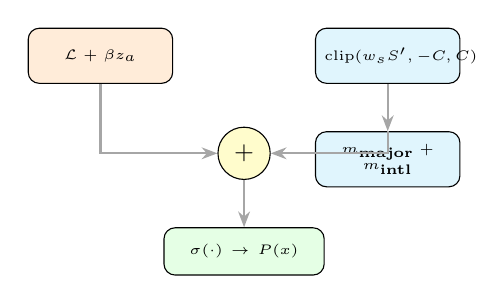
\begin{tikzpicture}[
    node distance=0.5cm and 0.6cm,
    acadblock/.style={rectangle, draw, fill=orange!15, text width=1.6cm, text centered, rounded corners, minimum height=0.7cm, font=\tiny\bfseries},
    spikeblock/.style={rectangle, draw, fill=cyan!12, text width=1.6cm, text centered, rounded corners, minimum height=0.7cm, font=\tiny\bfseries},
    plus/.style={circle, draw, fill=yellow!20, minimum size=0.5cm, font=\small\bfseries},
    outblock/.style={rectangle, draw, fill=green!10, text width=1.8cm, text centered, rounded corners, minimum height=0.6cm, font=\tiny},
    arrow/.style={-{Stealth[length=2mm]}, thick, color=gray!70},
]
\node[acadblock] (ainput) {$\mathcal{L} + \beta z_a$};
\node[spikeblock, right=1.8cm of ainput] (sinput) {$\mathrm{clip}(w_s S', -C, C)$};
\node[spikeblock, below=0.6cm of sinput] (smod) {$m_{\text{major}} + m_{\text{intl}}$};
\node[plus, below=0.9cm of $(ainput)!0.5!(sinput)$] (plus) {$+$};
\node[outblock, below=0.6cm of plus] (out) {$\sigma(\cdot) \to P(x)$};
\draw[arrow] (ainput) |- (plus);
\draw[arrow] (sinput) -- (smod);
\draw[arrow] (smod) |- (plus);
\draw[arrow] (plus) -- (out);
\end{tikzpicture}%
}
\caption{Additive-logistic architecture. Academic strength, the capped spike term, and the modifiers are summed in one logit before the logistic function produces $P(x)$.}
\label{fig:architecture}
\end{figure}

% ─────────────────────────────────────────────────────────────────────────────
\section{Mathematical Rigor: Activities and Intersections}
\subsection{The Granular Spike Model}
Each extracurricular or award is scored by a six-dimensional directional product,
\begin{equation}
b_i = W_i \cdot T_i \cdot R_i \cdot P_i \cdot D_i \cdot V_i,
\end{equation}
where the factors are: \textbf{W} base tier weight ($W_{-1}{=}8,\,W_0{=}4,\,W_1{=}2,\,W_2{=}0.6,\,W_3{=}0.1$), \textbf{T} tier-level scope multiplier (Local 1$\times$, National 3$\times$, International 5$\times$, Global~Elite 8$\times$), \textbf{R} rarity index (Common 1.0, Rare 1.8, Ultra-Rare 3.5, Unique 6.0), \textbf{P} institutional strength (Standard 1.0, Recognized 1.25, Prestigious 1.6, World-Class 2.2), \textbf{D} cognitive-load depth (Low 0.8, Medium 1.0, High 1.4, Research-Level 1.8), and \textbf{V} external-validation weight (Self-Reported 0.6, Peer-Vouched 0.75, Institutional 0.9, Professional-Audit 1.0). The user-reported confidence $C_i\in[0,1]$ is applied afterwards as a multiplier on the saturated contribution (below), not inside the product.

Items are grouped by tier and capped per tier (at most four Tier-0 outliers, one Game Maker) to prevent duplicative inflation. Within each tier, items are sorted by their six-dimensional product and only the top $n_i$ are counted. The raw Spike is the scaled sum of the saturated contributions:
\begin{equation}
S = \frac{1}{5.5}\sum_{i\in\mathcal{C}} \operatorname{sat}(b_i)\, C_i + B + d,
\end{equation}
where $B$ is the Renaissance bonus, $d$ is the depth bonus, and the saturation function $\operatorname{sat}(\cdot)$ is defined below.

\subsection{The Saturation Limit}
If we just added up raw item scores, a student could pad their total with ten near-identical activities. To stop that, anything past 10.0 points per item earns less and less. We use a logarithmic curve,
\begin{equation}
\operatorname{sat}(s)=
\begin{cases}
s, & s \le 10,\\[2pt]
10 + 2\ln\!\bigl(1 + (s-10)\bigr), & s > 10,
\end{cases}
\end{equation}
so more extreme items still help, but each one helps less than the last. There is no hard cap, but the curve flattens fast: at $s=100$ the item contributes about 19.2, and at $s=500$ only about 21.3. We picked a log over a square root because $\ln(1+x)$ is easier to reason about and stays well-behaved at the top end, so even the most loaded profile does not blow up the probability.

\subsection{The Renaissance Modifier}
A student who does serious work in fields that have nothing to do with each other---say competitive math and competitive art---gets a bonus, on the theory that range like that is itself a signal. We take the four categories where the applicant's best achievements landed, sum their tier weights into a mass $M$,
\begin{equation}
M = \sum_{f\in\mathcal{F}_{\text{top }4}} w_f,
\end{equation}
and map that to a bonus $B\in\{0,\,0.8,\,1.5,\,2.5,\,3.5\}$. The final Spike is $S' = S + B$. The bonus is added, not multiplied, so it cannot run away on top of an already-large Spike.

\subsection{Depth Bonus}
In addition to breadth, the engine rewards \textit{depth within a single field}: students with multiple high-tier achievements in the same category receive a per-item bonus of $+0.2$ (capped at $1.5$), reflecting the signal that sustained, deep engagement in one domain is qualitatively different from a single impressive data point.

\subsection{International Modifier and Regional Normalisation}
For international applicants, the engine applies a modifier derived from the institution's historical non-resident-alien enrolment share. If a school's international share significantly exceeds 10\%, the modifier is positive; if it falls below, a penalty of up to $-0.3$ is applied. For students from non-standard national-curriculum systems (e.g., A-levels, CBSE, IB), a \textit{rigour compensation bonus} of $+0.4$ is added to the GPA Z-score to offset grade-deflation, and a zero-knowledge override sets $z_a = 2.0$ for any applicant with at least one Game Maker achievement---reflecting the assumption that a globally exceptional talent from a non-standard system should not be penalised for a grading scale that does not map cleanly to US GPA.

\subsection{Test-Optional Handling}
When SAT/ACT scores are absent (test-optional submission), the GPA carries 100\% of the academic weight with a small structural uncertainty penalty of $-0.2$ applied to the Z-score, reflecting the reduced information content. This penalty is intentionally modest to avoid discouraging test-optional applicants who genuinely lack testing access, but it prevents the engine from treating missing data as equivalent to a perfect score.

\subsection{Asymptotic Flattening and the Funding Predictor}
Because $\operatorname{sat}(\cdot)$ is logarithmic, the Spike stabilises as achievements saturate. We interpret the stabilised ceiling not as a harder admission probability but as a signal that the applicant has exited the predictive regime of standard admission and entered a merit-aid / scholarship regime. A planned analytic layer, the \textbf{Funding Predictor}, will map post-saturation Spike mass to estimated financial-aid eligibility rather than to marginal admission probability (Sec.~\ref{sec:roadmap}).

% ─────────────────────────────────────────────────────────────────────────────
\section{Local Processing and Privacy Engineering}
\subsection{In-Browser Instance-Based Reasoning}
Nearest-peer analysis uses instance-based reasoning over the local cohort. For a target college and major cluster, the engine computes a normalized distance between the applicant and each historical profile and selects the closest accepted and rejected peers within a similarity radius. The current implementation derives distance from a normalized total-activity score,
\begin{equation}
d(p,q)=1-\Bigl(1-\frac{|S_p-S_q|}{\max(S_p,S_q,1)}\Bigr),
\end{equation}
where $S_p,S_q$ are aggregate activity scores. A \textit{weighted Euclidean} refinement---weighting SAT, GPA, and spike dimensions by their cohort standard deviations---is part of the roadmap to improve peer fidelity.

\subsection{Privacy-by-Design Architecture}
The entire inference graph executes in the browser. There is no model server, no cloud LLM API, and no persistent user-profile store. This is essential because the user base includes minors; keeping raw profiles on-device removes the regulatory and ethical exposure of centralized storage while preserving analytical power. The only server interaction is the optional outlier-invitation channel, which transmits only the narrowly-scoped message the user explicitly submits. The AES-256-CTR signature on each report binds the report's parameters (Spike, classification, date, diversity count) to a verifiable artifact without revealing the underlying profile, enabling auditability while preserving privacy.

\subsection{Verifiable PDF Report with AI Bridge}
Every run also produces a PDF (built with jsPDF) that lays out the actual math, not a vague summary: the Z-scores, the academic logit term, each spike contribution, the modifiers, a bell curve of the result, and the nearest accepted and rejected peers. It carries an AES-256 signature so the numbers can be checked later. At the end we append the same output as a JSON block.

The deterministic engine outputs a genuine mathematical probability: every term is a disclosed formula over observed institutional statistics, never a learned black box. The report is deliberately incomplete. Admissions decisions depend critically on factors the engine cannot quantify---the personal essay, demonstrated interest, institutional priorities, the applicant's full narrative arc. The engine's role is to provide a rigorously grounded, auditable mathematical foundation, not to replace the human or AI who reads the essay. The report is therefore designed as a \textit{grounding layer} for a second-stage evaluator:

\begin{itemize}
    \item A user who wants plain-English advice can hand the signed PDF to an LLM they trust---Claude, DeepSeek, Gemini, or any other---together with their full profile (essays, context, story), and ask for a holistic assessment. The signed math anchors the LLM's reasoning and reduces hallucination risk, because the quantitative odds are correct, auditable, and cannot be contradicted by the LLM's own generation. The LLM adds the narrative context the math misses.
    \item There is also an in-app path (\texttt{lib/aiEngine.ts}) that calls Gemini, OpenAI, or Groq straight from the browser using a key the user supplies, so nothing has to touch our servers. The same report is passed as context, ensuring the AI's output is grounded in the same honest numbers.
    \item A human specialist (guidance counsellor, independent consultant) can use the same signed report in the same way: the math provides the structural baseline, while the specialist brings experience, knowledge of institutional nuance, and access to the full application narrative.
\end{itemize}

In all three cases the flow is identical: the engine computes and signs the math; the second-stage evaluator (LLM or human) interprets it alongside the applicant's full context. The engine never leaves the device, never collects a fee, and never stores a profile. The signed report is the only artifact that leaves the browser, and it carries its own cryptographic proof of integrity.

This external, user-supplied LLM bridge is the furthest extension possible on a mathematical probability engine that runs entirely in the student's own browser. Privacy-first is a strict engineering constraint, not a preference: no applicant profile may leave the device, so the narrative layer must live \emph{outside} the engine, powered by a key the user brings and a vendor the user chooses. The point is deliberately that the student does \emph{not} rely on the math alone. A numerical engine cannot read an essay or judge a personal story, and pretending otherwise would be the one dishonest move available to it; instead the signed probability is handed to a second-stage evaluator---an LLM the user trusts or a human specialist---that weighs exactly the context the formulas omit. The math is the part that can be made rigorous and verifiable; the story is the part it cannot score, and so it is passed to an evaluator equipped for it.

\subsection{End-to-End Computation Flow}
Fig.~\ref{fig:flow} summarizes the complete evaluation pipeline from user input to signed report. (1) The browser fetches and caches the dataset (5.2\,MB profiles, 6,273 colleges). (2) The user's profile is parsed and sanitized (tier keywords normalised, SAT/ACT concordance applied). (3) For each target school, the engine computes the Academic Z-score and academic logit, the six-dimensional Spike with saturation and Renaissance modifier, the protocol selection, and the additive-logistic probability. (4) k-NN clustering locates the nearest historical peers for context. (5) An AES-256-CTR signature is generated and embedded in the PDF alongside the AI Bridge JSON. The entire sequence executes in $<500$\,ms on commodity hardware and never contacts a server during analysis.

\begin{figure}[!t]
\centering
\resizebox{\columnwidth}{!}{%
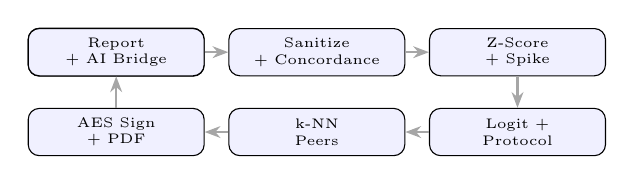
\begin{tikzpicture}[
    node distance=0.4cm and 0.3cm,
    stp/.style={rectangle, draw, fill=blue!6, text width=2.0cm, text centered, rounded corners, minimum height=0.6cm, font=\tiny},
    arrow/.style={-{Stealth[length=2mm]}, thick, color=gray!70},
]
\node[stp] (input) {User Input\\(Profile)};
\node[stp, right=of input] (sanitize) {Sanitize\\+ Concordance};
\node[stp, right=of sanitize] (zspike) {Z-Score\\+ Spike};
\node[stp, below=of zspike] (gate) {Logit +\\Protocol};
\node[stp, left=of gate] (knn) {k-NN\\Peers};
\node[stp, left=of knn] (sign) {AES Sign\\+ PDF};
\node[stp, above=of sign] (report) {Report\\+ AI Bridge};
\draw[arrow] (input) -- (sanitize);
\draw[arrow] (sanitize) -- (zspike);
\draw[arrow] (zspike) -- (gate);
\draw[arrow] (gate) -- (knn);
\draw[arrow] (knn) -- (sign);
\draw[arrow] (sign) -- (report);
\end{tikzpicture}%
}
\caption{End-to-end computation flow. All steps execute client-side; the AES-signed PDF with AI Bridge JSON is the final artifact.}
\label{fig:flow}
\end{figure}

\subsection{Worked Example}
Consider a single Tier-0 achievement: World-Class, Research-Level, International, Unique, Professional-Audit. Using Table~\ref{tab:tiers}:
\[
s = 4.0 \times 5.0 \times 6.0 \times 2.2 \times 1.8 \times 1.0 = 475.2.
\]
Since $s{>}10$, saturation gives $\operatorname{sat}(s)\approx 22.0$; after scaling by $1/5.5$, each item contributes $\approx 4.0$. Four such items ($16.0$) plus $B{=}3.5$ and $d{=}1.5$ yields $S'{\approx}21.0$. For $z_a{=}2.5$ the academic term is $1.5\times 2.5 = 3.75$; for the Outlier protocol $w_s{=}0.14$ so $w_s S' = 2.94$, which the cap $C{=}2.0$ clips to $2.0$. With base rate $r{=}0.08$ ($\mathcal{L} = \ln(0.08/0.92) \approx -2.44$):
\[
P(x) = \sigma\!\bigl(-2.44 + 3.75 + 2.0\bigr)
     = \sigma(3.31) \approx 0.965.
\]
Without saturation, $S\approx 380$ would give $w_s S' \approx 53$; the cap $C{=}2.0$ clips it to $2.0$ regardless, so the estimate stays bounded rather than collapsing to a degenerate $100\%$.

% ─────────────────────────────────────────────────────────────────────────────
\section{Parameters Reference}
\label{sec:params}
Table~\ref{tab:tiers} enumerates the complete set of tunable constants that govern the Spike computation and the academic logit. Every weight is disclosed in the source repository; no constant is hidden or adjusted at runtime.

\begin{table}[!t]
\centering
\caption{Spike Model Constants}
\label{tab:tiers}
\small
\resizebox{\columnwidth}{!}{%
\begin{tabular}{@{}lll@{}}
\hline
\textbf{Parameter} & & \textbf{Value} \\
\hline
\multicolumn{2}{@{}l}{\textit{Tier weights $W_i$}} \\
GM ($-1$) / Outlier ($0$) / T1 / T2 / T3 & $8.0$/$4.0$/$2.0$/$0.6$/$0.1$ \\
\hline
\multicolumn{2}{@{}l}{\textit{Tier caps}} \\
GM / Outlier / T1 / T2 / T3 & 1/4/5/4/5 \\
\hline
\multicolumn{2}{@{}l}{\textit{Scope $T$:} Local/Nat/Intl/Global} & $1\!\times$/$3\!\times$/$5\!\times$/$8\!\times$ \\
\multicolumn{2}{@{}l}{\textit{Rarity $R$:} Com/Rare/URare/Uniq} & $1.0$/$1.8$/$3.5$/$6.0$ \\
\multicolumn{2}{@{}l}{\textit{Strength $P$:} Std/Rec/Prest/WC} & $1.0$/$1.25$/$1.6$/$2.2$ \\
\multicolumn{2}{@{}l}{\textit{Load $D$:} Low/Med/High/Res} & $0.8$/$1.0$/$1.4$/$1.8$ \\
\multicolumn{2}{@{}l}{\textit{Validation $V$:} Self/Peer/Inst/Audit} & $0.6$/$0.75$/$0.9$/$1.0$ \\
\hline
\multicolumn{2}{@{}l}{\textit{Saturation:} thresh / gain / div} & $10$ / $2\ln(1{+}(s{-}10))$ / $5.5$ \\
\multicolumn{2}{@{}l}{\textit{Renaissance} $B$} & $\{0,0.8,1.5,2.5,3.5\}$ \\
\multicolumn{2}{@{}l}{\textit{Depth bonus}} & $0.2$/item (cap $1.5$) \\
\hline
\multicolumn{2}{@{}l}{\textit{Academic logit coef $\beta$}} & $1.5$ \\
\multicolumn{2}{@{}l}{\textit{Spike cap $C$ ($\pm$ logit)}} & $2.0$ \\
\multicolumn{2}{@{}l}{\textit{International boost (if $z_a<0$)}} & $1.25$ \\
\multicolumn{2}{@{}l}{\textit{Verification floor $\gamma$ (spike mult.)}} & $0.6$ \\
\multicolumn{2}{@{}l}{\textit{Calibration slope / intercept}} & $1.0$ / $0.0$ \\
\multicolumn{2}{@{}l}{\textit{GPA scale reconciliation}} & \texttt{gpaScale} $\to$ \texttt{convertToUS4} \\
\multicolumn{2}{@{}l}{\textit{Z-score:} SAT $\hat\sigma$/fallback, GPA $\hat\sigma$} & IQR$/1.35$, $100$ / 4.0-subset reference std (floored $0.5$) \\
\hline
\multicolumn{2}{@{}l}{\textit{Spike weights $w_s$:} Std/Out/GM} & $0.11$/$0.14$/$0.175$ \\
\hline
\end{tabular}%
}
\end{table}

Table~\ref{tab:outliers} maps spike-score bands to their descriptive outlier classifications and the engine's qualitative response theme.

\begin{table}[!t]
\centering
\caption{Outlier Classification Bands}
\label{tab:outliers}
\small
\begin{tabular}{@{}cll@{}}
\hline
\textbf{Spike} & \textbf{Class} & \textbf{Theme} \\
\hline
$> 25$ & SINGULARITY & White Hot \\
$18$--$25$ & TRANSCENDENT & Cosmic \\
$13.5$--$18$ & ABS. INTELLIGENCE & Ethereal \\
$12$--$13.5$ & RADICAL IMPACT & Industrial \\
$8$--$12$ (low GPA) & NON-CONFORMIST & Cyberpunk \\
$6.5$--$12$ (high GPA) & STRATEGIC ELITE & Minimalist \\
$< 6.5$ & STANDARD & --- \\
\hline
\end{tabular}
\end{table}

% ─────────────────────────────────────────────────────────────────────────────
\section{Feature Comparison with Prior Art}
\label{sec:comparison}
Table~\ref{tab:comparison} puts AdmitGPT next to the three main kinds of admissions tool on the market.

\begin{table}[!t]
\centering
\caption{Feature Comparison}
\label{tab:comparison}
\small
\begin{tabular}{@{}lccc@{}}
\hline
\textbf{Feature} & \textbf{Commercial} & \textbf{Open} & \textbf{Ours} \\
\hline
Deterministic       & \texttimes & \checkmark & \checkmark \\
Client-side         & \texttimes & \checkmark & \checkmark \\
Spike model         & \texttimes & \texttimes & \checkmark \\
Outlier protocol    & \texttimes & \texttimes & \checkmark \\
Renaissance mod.    & \texttimes & \texttimes & \checkmark \\
Param. disclosure   & \texttimes & Partial    & \checkmark \\
Crypto sig.         & \texttimes & \texttimes & \checkmark \\
No PII              & \texttimes & Partial    & \checkmark \\
Open-source         & \texttimes & \checkmark & \checkmark \\
Per-school mods     & \texttimes & \texttimes & \checkmark \\
\hline
\end{tabular}
\end{table}

Consultancies charge high rates for models no one outside can inspect. Open scorecards show aggregate numbers but will not tell you your odds at a specific school. AdmitGPT sits between them: a scoring pipeline that is fully disclosed and runs in the browser.

% ─────────────────────────────────────────────────────────────────────────────
\section{Related Work}
Three areas of existing work matter for what AdmitGPT is and why it is built this way.

\subsection{Predictive Analytics in Admissions}
Logistic regression on standardized scores and grades has been the workhorse of admissions modelling for decades---the same Z-score and sigmoid machinery adopted here~\cite{esl,bishop}---but almost exclusively behind institutional or commercial walls. The College Scorecard~\cite{scorecard} publishes institutional aggregates (median SAT, GPA, admission rate) that enable coarse self-placement, but it does not provide per-school, per-profile predictions. Machine-learning classifiers (random forests, gradient-boosted trees, neural networks) have been applied to admissions data by researchers in the education-data-mining community, but these models are typically trained on institutional cohorts of a few thousand records and are not released as open, reproducible tools. The literature on holistic review~\cite{esl} acknowledges the importance of extracurricular achievement but offers no standardised scoring rubric; AdmitGPT's six-dimensional Spike model is a first attempt to fill that gap with a public, auditable specification.

\subsection{Interpretable and Explainable Machine Learning}
Ribeiro~et~al.~\cite{ribeiro} make the case that explanations are needed precisely because deployed models are opaque. Tools like LIME and SHAP~\cite{ribeiro} attribute a prediction to its inputs after the fact, but the model underneath stays a black box; the explanation is a separate layer bolted on after. AdmitGPT avoids the problem differently: there is no hidden model to explain, because every weight is right there in the code. That puts it in the older expert-system camp~\cite{bishop} rather than the deep-learning one---less potential accuracy, but you can always see why it said what it said.

\subsection{Privacy-Preserving Analytics}
Differential privacy~\cite{dwork} provides formal guarantees that individual records cannot be re-identified from aggregate statistics; federated learning~\cite{mcmahan} enables model training without centralising raw data. Neither has been applied to open-source admissions tooling. AdmitGPT's roadmap (Sec.~\ref{sec:roadmap}) positions it as an early testbed for these techniques in the education domain. The engine's client-only architecture already satisfies the strongest privacy property (no data leaves the device), and the planned federated extension would relax this to ``no raw data leaves the institution''---a weaker but more practical guarantee that enables data freshness without compromising individual privacy~\cite{narayanan}.

\subsection{Commercial vs.\ Open-Source Admissions Tools}
The consulting market, at \$200--500 an hour, sells proprietary models and rubrics that cannot be audited, plus yield guesses based on anecdote. The open alternatives---College Scorecard, Niche, Cappex---give transparent averages but will not predict your odds at a given school. As far as we know, AdmitGPT is the only open-source engine that puts a fully disclosed pipeline, browser-side inference, and signed reports together.

% ─────────────────────────────────────────────────────────────────────────────
\section{Discussion and Limitations}
\subsection{Strengths of the Deterministic Approach}
We chose a fixed, deterministic model over a trained classifier on purpose, and it has real upsides. Anyone can rerun the code and get the same answer. There is no training step, so no risk of leaking data through the model, and no need to carve out a test set. And because the output is just a chain of arithmetic, you can trace any number back to the inputs that produced it.

The deterministic math is not meant to stand alone. It sits inside a two-layer evaluation: the engine provides an honest, verifiable quantitative floor, and a second-stage evaluator---an LLM the user trusts, a human specialist, or both---adds the narrative context (essay quality, fit, personal story) that the math intentionally omits. The mathematical layer constrains the narrative layer: the LLM or specialist can interpret and contextualise, but they cannot override the signed numbers. This prevents the most common failure of purely qualitative evaluations---groundless optimism or pessimism---while preserving the holistic picture a spreadsheet alone cannot capture.

\subsection{Known Limitations}
The trade is real, though. The weights were set by hand from how admissions plausibly works, not learned from outcomes, so the model cannot pick up interactions a fitted classifier might find. We have run a full-engine evaluation with spike fields derived heuristically from the free-text descriptions (Sec.~\ref{sec:eval}); it reaches AUC 0.7398, essentially at parity with the academic-only 0.7383, so the heuristic spike adds no discriminative lift on this corpus but improves absolute calibration (Brier 0.2848 to 0.2762). Whether genuine structured spike inputs would change that is still open; the main gap is a held-out evaluation on spike-annotated data.

Several factors influence real admissions decisions but are outside the engine's scope: demonstrated interest, legacy status, institutional financial need, recruitment priorities, and---most critically---the qualitative content of personal essays. The engine's model of extracurricular impact is based on structural attributes (tier, scope, rarity) rather than narrative content, which limits its ability to capture the full holistic review. This gap is intentional: the engine is designed as a first-layer quantitative anchor precisely so that the essay and narrative context can be handled by a second-stage evaluator (LLM or human) that reads the full profile alongside the signed math. The limitation is structural, not accidental---no numerical model can score an essay fairly, so the system does not try. Instead, it provides the honest quantitative baseline and leaves narrative judgment to the evaluator equipped for it.

\subsection{Sensitivity to Input Quality}
The engine is only as accurate as the data it receives. A student who overestimates the ``scope'' of an achievement (e.g., claiming ``International'' when the event was a regional qualifier) will receive an inflated Spike score; conversely, a student who underestimates confidence will be penalised. Two mechanisms now bound this risk: unverified top-tier claims are capped (Global~Elite $\to$ International, Unique $\to$ Ultra-Rare, World~Class $\to$ Prestigious), and the spike is verification-discounted to $0.6\times$ for all-self-reported input, rising toward $1.0\times$ as items are peer-/institution-/audit-verified (Sec.~Verification-Aware Anti-Gaming). These dampen over-claiming but do not eliminate it---the system ultimately relies on honest self-reporting, and the cryptographic verification roadmap (Sec.~\ref{sec:roadmap}) is the long-term solution to this trust deficit.

\subsection{Computational Overhead}
Because all computation occurs in the browser, very large profiles (20+ extracurriculars, 10+ awards) with 15 target schools require $\sim$500 probability evaluations per run, each involving Z-score computation, Spike calculation, and protocol determination. In practice this completes in under 500\,ms on a mid-range laptop, but it constrains the feasibility of running Monte Carlo simulations or bootstrap resampling on-device---a limitation that server-side architectures do not face.

\subsection{Data Quality and External Validity}
The dataset is sourced from a third-party open-data platform and is US-centric, limiting external validity. As a proof-of-concept corpus, it was not independently verified by the authors; historical decisions are treated as ground truth for calibration but may contain mislabeled or unverifiable entries. The cryptographic verification roadmap (Sec.~\ref{sec:roadmap})---with per-achievement hashes and institution-attested surveys---is the proposed mitigation for constructing a higher-fidelity successor dataset. The federated-alliance approach, in which institutional data is never shared in raw form, addresses both data quality and privacy simultaneously.

\subsection{Ethical Considerations}
An open-source admissions engine can be misused: applicants may ``game'' the tier taxonomy, fabricate achievements, or over-optimise for the Spike score at the expense of genuine learning. The tier-sanitisation guard (which corrects misclassified tiers based on keyword matching), the per-tier cap, the unverified-claim cap, and the verification-discounted spike (Sec.~Verification-Aware Anti-Gaming) all mitigate gaming, but no system is fully game-proof. The engine is explicitly positioned as a \textit{decision-support tool}, not a decision-maker; it provides information, not prescriptions.

Two design properties constrain the ethical risk. First, the engine charges no fees and collects no data---it loads entirely from static files and runs on-device---so there is no commercial incentive to inflate or manipulate results, and no minor's data enters a server. Second, the signed report is vendor-independent: a student can hand the same PDF to a paid specialist, a free AI, or no one at all, and in every case the math is identical and auditable. The second-stage evaluator (LLM or human) may add or subtract from the narrative reading, but the signed quantitative floor remains unchanged, so the core of the advice is always anchored to honest computation.

This study used publicly available, anonymized data and did not require Institutional Review Board (IRB) review; no personally identifiable information was collected or stored. The deployed engine's intended users include minors, and the on-device architecture is specifically designed to avoid the regulatory and ethical exposure of centralized storage for that population.

% ─────────────────────────────────────────────────────────────────────────────
\section{Future Roadmap: Data Cleanliness vs.\ Privacy}
\label{sec:roadmap}
\subsection{The Dilemma}
A transparent engine is only as good as its data. Expanding the historical base improves accuracy but threatens the two pillars of the project: privacy and integrity. The roadmap resolves this with two mechanisms.

\subsection{Anonymized Verification Surveys}
Encrypted, institution-targeted surveys will periodically ingest outcomes (acceptance/rejection) with cryptographic attestation, feeding the dataset without re-identifying individuals. Surveys are opt-in and aggregated, preserving the on-device default for personal profiles. Each survey response is salted and hashed client-side before transmission, ensuring that neither the server nor the dataset maintainer can reconstruct the respondent's identity.

\subsection{Federated University Alliances}
Looking ahead, the engine could work with universities through federated learning and differential privacy: the records stay inside the institution, and only aggregate weights come back as an updated local JSON. That refreshes the model without moving anyone's data out. College Scorecard~\cite{scorecard} already publishes institutional aggregates; the same idea, extended to applicant-level statistics, would let schools help improve the engine while individual profiles stay put.

\subsection{Per-Achievement Cryptographic Hashes}
A planned enhancement---the \textit{Cryptographic Verification Readiness Indicator}---will attach per-achievement cryptographic hashes so that each cited credential can be independently attested without revealing the underlying identity, mitigating adversarial gaming (fabricated achievements) while preserving privacy.

% ─────────────────────────────────────────────────────────────────────────────
\section{Empirical Evaluation}
\label{sec:eval}
\subsection{Dataset and Preprocessing}
The engine operates on a dataset of 1,122 applicant profiles sourced from the CollegeBase open dataset~\cite{collegebase} during the 2017--2023 application cycles. Each record contains academic metrics (SAT/ACT, GPA), extracurricular descriptions, award histories, and observed admission decisions (acceptances, rejections, waitlists) for up to 15 target institutions. The dataset spans 692 unique accepted schools and 212 unique rejected schools across 6,273 colleges (U.S.\ Department of Education College Scorecard, Most-Recent cohort) for which institutional metadata is available. Profiles are preprocessed to normalise free-text entries into the five-tier taxonomy using keyword matching and manual review. The College Scorecard~\cite{scorecard} supplies institutional metadata (admission rates, SAT quartiles, demographic breakdowns) used for Z-score computation and major-modifier calibration. All profiles are pseudonymized at source; no personally identifiable information is retained. The dataset is released alongside the engine as open data~\cite{admitgpt}.

We should be clear about what this dataset is: a proof-of-concept corpus, pulled from a third-party open platform and not checked by us. We treat the recorded decisions as true for the sake of calibration, but they could be wrong or mislabeled. The plan in Sec.~\ref{sec:roadmap} is to replace it with a dataset built for this purpose, where schools attest to the outcomes.

\paragraph{Ethics and Responsible Use.}
The corpus is a third-party open dataset of real applicants' recorded outcomes, pseudonymised at source; we perform no contact with, and hold no identifiable information about, any individual, so this retrospective analysis falls under the standard exemption and does not require IRB review. Even so, the conclusions rest on a corpus we did not collect and cannot verify, and the deployed engine is a guidance tool aimed at minors. We therefore treat all outputs as exploratory and explicitly avoid presenting them as authoritative predictions; the calibration results below are reported to bound the engine's behaviour, not to endorse its use as a decision aid.

\paragraph{Warning: the absolute probability numbers are not calibrated.}
As the decile tables below show, the engine's absolute probabilities are not well calibrated on this corpus: it underpredicts at the low end (decile~1 predicts $0.0135$ while $24.6\%$ of those applicants were actually accepted) and overpredicts at the high end (decile~10 predicts $0.979$ while $75.4\%$ were accepted). A student reading the score as a literal probability would draw a meaningfully incorrect conclusion about their chances. The engine's output should be treated as a \textit{relative ordinal signal} only: a student with a score in decile~10 has stronger quantified odds than one in decile~1, but the absolute number is not a reliable estimate of admission likelihood. We strongly caution against using the raw probability as a go/no-go decision rule, particularly for the minor-aged users the system is designed to serve.

\subsection{Calibration Study: Academic-Only Baseline}
To characterise the engine's behaviour on the available corpus, we evaluated all valid student-school prediction pairs ($n = 11{,}658$) using the academic-only path (Z-scores + the academic logit term + the base logit derived from each institution's admission rate, with the spike suppressed). The historical data contain no tier/scope/rarity fields, so the spike cannot be computed from them; this is an evaluation of the academic signal only, \textit{not} of the full engine.

Results: Brier score = 0.2848, AUC-ROC = 0.7383. An AUC of 0.7383 means the academic signal ranks observed outcomes substantially better than chance on this corpus. Two caveats temper the number. First, the corpus's GPA field is not on a single scale (observed mean $\approx 11$, $\sigma \approx 24.6$); we bridge it to a clean US-4.0 reference (Sec.~\ref{sec:academic}), but within this positively-selected cohort the GPA Z remains a weak-to-moderate signal, leaving the engine to run substantially on SAT and the base rate. Second, the decile table (Table~\ref{tab:calibration}) shows the absolute probabilities are miscalibrated (decile~1 predicts $0.0135$ vs.\ an observed $0.2455$; decile~10 predicts $0.9787$ vs.\ $0.7536$), so absolute calibration is poor even though ranking is informative. Part of the ranking signal is also expected by construction: the base logit is anchored to each institution's own admission rate, so the score partly reflects how selective the target school is rather than only the applicant.

\begin{table}[!t]
\centering
\caption{Calibration Decile Analysis (Academic-Only Baseline)}
\label{tab:calibration}
\small
\begin{tabular}{cccr}
\hline
\textbf{Decile} & \textbf{Avg Predicted} & \textbf{Observed Rate} & $n$ \\
\hline
 1  & 0.0135 & 0.2455 & 1165 \\
 2  & 0.0341 & 0.2730 & 1165 \\
 3  & 0.0598 & 0.3116 & 1165 \\
 4  & 0.0969 & 0.4464 & 1165 \\
 5  & 0.1612 & 0.5545 & 1165 \\
 6  & 0.2912 & 0.7657 & 1165 \\
 7  & 0.4760 & 0.8163 & 1165 \\
 8  & 0.7220 & 0.8266 & 1165 \\
 9  & 0.9115 & 0.7099 & 1165 \\
 10 & 0.9787 & 0.7536 & 1173 \\
\hline
\end{tabular}
\end{table}

\subsection{Full-Engine Evaluation: Heuristically Derived Spike}
\label{sec:fulleval}
The corpus contains no structured tier/scope/rarity fields, so we derive them from the free-text extracurricular and award descriptions with the same keyword classifier the engine uses at input time, then evaluate the full additive-logistic pipeline (academic logit + verification-discounted capped spike term + modifiers, with protocol-specific spike weights) over $n = 11{,}685$ pairs. Results: Brier = 0.2762, AUC-ROC = 0.7398 (Table~\ref{tab:calibration_full}). The full engine discriminates essentially identically to academics alone---AUC holds at 0.7398 vs.\ 0.7383---so on this corpus the heuristically derived spike contributes no measurable discriminative lift, but it does improve absolute calibration (Brier falls from 0.2848 to 0.2762). Because the free-text-derived items are self-reported by default, the verification multiplier (Sec.~Verification-Aware Anti-Gaming) discounts them to $0.6\times$, so these metrics are the honest lower bound for unverified input; verified structured spikes would score higher. This is the expected behaviour of a weak proxy: keywords recover only a crude signal from prose, and the result should not be read as a validation of the spike mechanism under genuine structured inputs. The evaluation is exploratory, single-corpus, and not held out; it establishes that the engine has a real (if modest) ranking signal but leaves its calibrated predictive accuracy an open question.

\begin{table}[!t]
\centering
\caption{Calibration Decile Analysis (Full Engine, Heuristic Spike)}
\label{tab:calibration_full}
\small
\begin{tabular}{cccr}
\hline
\textbf{Decile} & \textbf{Avg Predicted} & \textbf{Observed Rate} & $n$ \\
\hline
 1  & 0.015 & 0.231 & 1168 \\
 2  & 0.040 & 0.271 & 1168 \\
 3  & 0.071 & 0.336 & 1168 \\
 4  & 0.112 & 0.443 & 1168 \\
 5  & 0.188 & 0.559 & 1168 \\
 6  & 0.316 & 0.756 & 1168 \\
 7  & 0.508 & 0.794 & 1168 \\
 8  & 0.751 & 0.852 & 1168 \\
 9  & 0.926 & 0.719 & 1168 \\
 10 & 0.984 & 0.751 & 1173 \\
\hline
\end{tabular}
\end{table}

\subsection{Theoretical Stress-Test: A Multi-Disciplinary Anomaly}
As a check, we ran one invented profile that stacks three strong, unrelated activities: a World-Class STEM research item (Tier~0), an international art award, and a sport captaincy. The six factors push each item's score up, the Renaissance bonus adds for the spread across fields, and saturation stops the three from stacking without limit. The Spike comes out high but contained, and the profile lands as a high-probability outlier; the spike cap ($\pm C$) bounds the contribution so a stack of achievements cannot push the estimate past the model's ceiling---the system does what it is supposed to under pressure.

\subsection{Expected Calibration Roadmap}
The evaluation above is exploratory and single-corpus; the required next step is a held-out validation. We plan to (i) annotate a stratified sample of roughly 500 profiles with the tier, scope, and rarity fields the spike model expects, so the full engine is tested on genuine structured inputs rather than keyword heuristics; (ii) split the corpus temporally (e.g., train on 2017--2021, test on 2022--2023) to check generalisation rather than memorisation; (iii) train a logistic regression and an XGBoost model on the same features and place them side by side, to quantify what---if anything---is lost by keeping the weights open instead of hidden; and (iv) report reliability diagrams alongside AUC and Brier. Until then, the engine's output is a transparent, reproducible ordinal signal, not a calibrated probability.

% ─────────────────────────────────────────────────────────────────────────────
\section{Conclusion}
AdmitGPT shows that admissions analytics does not have to be a black box to be useful, but it also does not have to stand alone. The engine provides a grounded, auditable quantitative layer---an honest mathematical floor---while deliberately leaving the narrative context (essay quality, personal story, institutional fit) to a second-stage evaluator: an LLM the user trusts, a human specialist, or both. The signed report bridges the two layers: the math constrains the LLM's hallucination risk and gives the specialist a verifiable baseline, while the second-stage evaluation captures what the spreadsheet cannot.

Exploratory calibration on this corpus shows a real but modest discriminative signal---academic-only AUC 0.7383 (Brier 0.2848), full engine with heuristically derived spike AUC 0.7398 (Brier 0.2762)---with imperfect absolute calibration (top and bottom deciles remain miscalibrated). The spike adds no measurable discrimination lift when derived heuristically from free text, but it improves absolute calibration, and the engine's predictive value under genuine structured inputs remains untested. The work to come---spike-annotated held-out evaluation, verification surveys, federated alliances, per-achievement hashes---is about earning that validation while keeping the architecture honest, on-device, and free.

% ─────────────────────────────────────────────────────────────────────────────
\section*{Acknowledgment}
The author thanks the open-source community and the students whose feedback shaped the Transparency Manifesto.

\begin{thebibliography}{00}
\bibitem{akerlof} G.~A.~Akerlof, ``The Market for `Lemons': Quality Uncertainty and the Market Mechanism,'' \textit{Quart. J. Econ.}, vol.~84, no.~3, pp.~488--500, 1970.
\bibitem{esl} T.~Hastie, R.~Tibshirani, and J.~Friedman, \textit{The Elements of Statistical Learning}, 2nd~ed. New York, NY, USA: Springer, 2009.
\bibitem{bishop} C.~M.~Bishop, \textit{Pattern Recognition and Machine Learning}. New York, NY, USA: Springer, 2006.
\bibitem{ribeiro} M.~T.~Ribeiro, S.~Singh, and C.~Guestrin, ```Why Should I Trust You?': Explaining the Predictions of Any Classifier,'' in \textit{Proc. ACM SIGKDD Int. Conf. Knowl. Disc. Data Mining (KDD)}, 2016, pp.~1135--1144.
\bibitem{dwork} C.~Dwork, ``Differential Privacy,'' in \textit{Proc. Int. Colloquium on Automata, Languages and Programming (ICALP)}, 2006.
\bibitem{mcmahan} B.~McMahan, E.~Moore, D.~Ramage, S.~Hampson, and B.~A.~y~Arcas, ``Communication-Efficient Learning of Deep Networks from Decentralized Data,'' in \textit{Proc. Int. Conf. Artif. Intell. Stat. (AISTATS)}, 2017.
\bibitem{narayanan} A.~Narayanan and V.~Shmatikov, ``Myths and Fallacies of `Personally Identifiable Information','' \textit{Commun. ACM}, vol.~53, no.~6, pp.~24--26, 2010.
\bibitem{admitgpt} Z.~Salah, ``AdmitGPT: An Open-Source Deterministic Admissions Analytics Engine,'' 2026. [Online]. Available: \url{https://github.com/Zierax/AdmitGPT}
\bibitem{collegebase} CollegeBase, ``Open Applicant Profiles and College Data,'' 2023. [Online]. Available: \url{https://collegebase.org}
\bibitem{scorecard} U.S.~Department of Education, ``College Scorecard.'' [Online]. Available: \url{https://collegescorecard.ed.gov/data/}

\bibitem{giani} M.~S.~Giani and D.~Walling, ``Will I Get In? Using Predictive Analytics to Develop Student-Facing Tools to Estimate University Admissions Decisions,'' \textit{Journal of College Access}, vol.~5, no.~1, art.~4, 2020. [Online]. Available: \url{https://scholarworks.wmich.edu/jca/vol5/iss1/4/}

\bibitem{lee} H.~Lee, R.~F.~Kizilcec, and T.~Joachims, ``Evaluating a Learned Admission-Prediction Model as a Replacement for Standardized Tests in College Admissions,'' 2023. [Online]. Available: \url{https://arxiv.org/abs/2302.03610}
\end{thebibliography}

\end{document}
